
\section{Công thức cộng xác suất}
\subsection{Công thức cộng xác suất cho hai biến cố xung khắc}

\subsubsection{Biến cố xung khắc}
\begin{dn}
	Biến cố $A$ và biến cố $B$ được gọi là \textbf{xung khắc} nếu $A$ và $B$ không đồng thời xảy ra.\\
	Hai biến cố $A$ và $B$ \textbf{xung khắc }khi và chỉ khi $A\cap B=\varnothing $.
\end{dn}
\begin{center}
	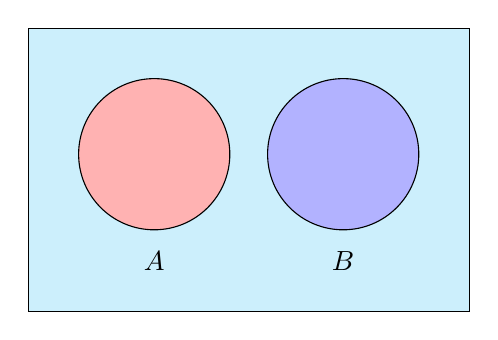
\begin{tikzpicture}[scale=0.8]
		\fill[color=cyan!20] (0,0.5) rectangle (7,5);
		\fill[color=red!30] (2,3) circle (1.2);
		\fill[color=blue!30] (5,3) circle (1.2);
		\draw (0,0.5) rectangle (7,5);
		\draw (2,3) circle (1.2);
		\draw (5,3) circle (1.2);
		\path (2,1.3) node{$A$} (5,1.3) node{$B$};	
	\end{tikzpicture}
\end{center}
\begin{vd}
	Gieo đồng thời hai con xúc xắc cân đối, đồng chất. Xét các biến cố sau:
	\begin{itemize}
		\item 	$A$: “Tổng số chấm xuất hiện trên hai con xúc xắc lớn hơn hoặc bằng $7$”;
		\item 	$B$: “Tổng số chấm xuất hiện trên hai con xúc xắc nhỏ hơn hoặc bằng $5$”;
		\item 	$C$: “Tổng số chấm xuất hiện trên hai con xúc xắc là số nguyên tố”.
	\end{itemize}
	Trong các cặp biến cố $A$ và $B$; $A$ và $C$ cặp biến cố nào xung khắc? Tại sao?
	\loigiai{
		Cặp biến cố $A$ và $B$ là xung khắc vì $A$ và $B$ không đồng thời xảy ra.\\
		Cặp biến cố $A$ và $C$ không xung khắc vì nếu tổng số chấm xuất hiện trên hai con xúc xắc bằng $7$ thì cả $A$ và $C$ xảy ra.}
\end{vd}

\subsubsection{Công thức cộng xác suất cho hai biến cố xung khắc}
\begin{dn}
	Nếu $A$ và $B$ là hai biến cố xung khắc thì
	\begin{align*}
		P(A\cup B)=P(A)+P(B).
	\end{align*}
\end{dn}
\begin{vd}
	Một hộp đựng $10$ tấm thẻ cùng loại được ghi số từ $1$ đến $10$. 
	Rút ngẫu nhiên đồng thời hai tấm thẻ từ trong hộp. Xét các biến cố sau:
	\begin{itemize}
		\item 	$A$: “Cả hai tấm thẻ đều ghi số chẵn”;
		\item $B$: “Chỉ có một tấm thẻ ghi số chẵn”;
		\item $C$: “Tích hai số ghi trên hai tấm thẻ là một số chẵn”.
	\end{itemize}
	Chứng minh rằng $C=A\cup B$.
	\loigiai{
		Biến cố $C$ xảy ra khi và chỉ khi trong hai tấm thẻ có ít nhất một tấm thẻ ghi số chẵn.\\
		Nếu cả hai tấm thẻ ghi số chẵn thì biến cố $A$ xảy ra. \\
		Nếu chỉ có một tấm thẻ ghi số chẵn thì biến cố $B$ xảy ra. \\
		Vậy $C$ là biến có hợp của $A$ và $B$.\\
		Hai biến cố $A$ và $B$ xung khắc. Do đó $P( C )=P( A\cup B )=P( A )+P( B )$.\\
		Ta cần tính $P( A )$ và $P( B )$. \\
		Không gian mẫu $\Omega $ là tập hợp tất cả các tập con có hai phần tử của tập $\{ 1;2;\cdot \cdot \cdot ;10 \}$.\\
		Do đó $ n( \Omega )=\mathrm{C}_{10}^2=45$.\\
		*Tính $P( A )$: Biến cố $A$ là tập hợp tất cả các tập con có hai phần tử của tập $\{ 2;4;6;8;10 \}$.\\
		Do đó $ n( A )=\mathrm{C}_2^5=10$. Suy ra $P( A )=\dfrac{n( A )}{n( \Omega )}=\dfrac{10}{45}=\dfrac{2}{9}$.\\
		*Tính $P( B )$: Mỗi phần tử của $B$ được hình thành từ hai công đoạn:\\
		Công đoạn 1: Chọn một số chẵn từ tập $\{ 2;4;6;8;10 \}$. Có $5$ cách chọn.\\
		Công đoạn 2: Chọn một số lẻ từ tập $\{ 1;3;5;7;9 \}$. Có $5$ cách chọn.\\
		Theo quy tắc nhân, tập $B$ có $5\cdot 5=25$ (phần tử).\\
		Do đó $ n( B )=25$. Suy ra $P( B )=\dfrac{n( B )}{n( \Omega )}=\dfrac{25}{45}=\dfrac{5}{9}$.\\
		Vậy $P( C )=P( A )+P( B )=\dfrac{2}{9}+\dfrac{5}{9}=\dfrac{7}{9}$.
	}
\end{vd}
\subsection{Công thức cộng xác suất}
\begin{dn}
	Cho hai biến cố $A$ và $B$. Khi đó, ta có:
	\begin{align*}
		P( A\cup B )=P( A )+P( B )-P( AB ).
	\end{align*}
	Công thức này được gọi là công thức cộng xác suất.
\end{dn}
\begin{vd} Ở một trường trung học phổ thông $X$, có $18\%$ học sinh học khá môn Ngữ văn,  $30\%$ học sinh học khá môn Toán, $6\%$ học sinh học khá cả hai môn  văn và Toán. Chọn ngẫu nhiên một học sinh của trường $X$. \\
	Xét hai biến cố sau:
	\begin{itemize}
		\item $A$: “Học sinh đó học khá môn Ngữ văn”;
		\item $B$: “Học sinh đó học khá môn Toán”.
	\end{itemize}
	a) Hoàn thành các mệnh đề sau bằng cách tìm cụm từ thích hợp thay cho dấu $?$
	\begin{itemize}
		\item $P( A )$ là tỉ lệ $?$
		\item $P( B )$ là $?$
		\item $P( AB )$ là $?$
		\item $P( A\cup B )$ là $?$
	\end{itemize}
	b) Hãy tính tỉ lệ học sinh học khá môn Ngữ văn hoặc học khá môn Toán của trường $X$.
	\loigiai{
		a)
		\begin{itemize}
			\item $P(A)$ là tỉ lệ học sinh học khá môn Ngữ văn của trường $X$.
			\item $P(B)$ là tỉ lệ học sinh học khá môn Toán của trường $X$.
			\item $P(AB)$ là tỉ lệ học sinh học khá môn Ngữ văn và Toán của trường $X$.
			\item $P(A\cup B)$ là tỉ lệ học sinh học khá môn Ngữ văn hoặc Toán của trường $X$.\\
		\end{itemize}
		b) Tỉ lệ học sinh học khá môn Ngữ văn hoặc học khá môn Toán của trường $X$ là
		$P( A\cup B )$.\\
		Ta có
		\begin{center}
			$P( A )=18\%=0{,}18$;  $P( B )=30\%=0{,}3$ và $P( AB )=6\%=0{,}06$.
		\end{center}
		Theo công thức cộng xác suất, ta có:
		\begin{align*}
			P( A\cup B )=P( A )+P( B )-P(AB )=0{,}18+0{,}3-0{,}06=0{,}42 .
		\end{align*}
		Do đó, xác suất để chọn ngẫu nhiên một học sinh của trường X học khá môn Ngữ Văn hoặc học khá môn Toán là $0{,}42$.\\
		Vậy tỉ lệ học sinh khá môn Ngữ Văn hoặc khá môn Toán của trường X là $42\%$. }
\end{vd}
\begin{dang}{Tính xác suất bằng định nghĩa}
		Một phép thử ngẫu nhiên có không gian mẫu là $\Omega$.\\
	Xác suất của biến cố $A$ kí hiệu là $P(A)$ và được tính theo công thức $P(A)=\dfrac{n(A)}{n(\Omega)}$.
\end{dang}



\subsubsection{Các ví dụ}
\begin{vd}
	Một hộp chứa $11$ quả cầu gồm $5$ quả màu xanh và $6$ quả cầu màu đỏ. Chọn ngẫu nhiên đồng thời $2$ quả cầu từ hộp đó. Xác suất để $2$ quả cầu chọn ra cùng màu bằng
	\choice
	{$ \dfrac{5}{22} $}
	{$ \dfrac{6}{11} $}
	{\True$ \dfrac{5}{11} $}
	{$ \dfrac{8}{11} $}
	\loigiai{
		Ta có $n(\Omega)=\displaystyle C^2_{11}=55$.\\
		Gọi biến cố $A$: "Chọn $2$ quả cầu cùng màu".\\
		Do đó $n(A)=\displaystyle C^2_5\cdot C^2_6=25$.\\
		Vậy xác suất của biến cố $A$ là $P(A)=\dfrac{n(A)}{n(\Omega)} =\dfrac{25}{55}=\dfrac{5}{11}$.
	}
\end{vd}
\begin{vd}
	Gieo đồng thời hai con xúc xắc cân đối và đồng chất. Xác suất để tổng số chấm xuất hiện của hai con xúc xắc đó không vượt quá $5$ bằng
	\choice
	{$ \dfrac{5}{12} $}
	{$ \dfrac{1}{4} $}
	{$ \dfrac{2}{9} $}
	{\True$ \dfrac{5}{18} $}
	\loigiai{
		Ta có $n(\Omega)=6^2=36$.\\
		Gọi $A$ là biến cố "Tổng số chấm của hai xúc xắc không vượt quá $5$".\\
		Khi đó, $A=\left\lbrace (1,1);(1,2);(1,3);(1,4); (2,1); (2,2);(2,3) (3,1);(3,2) (4,1)\right\rbrace$.\\
		Suy ra $n(A)=10$.\\
		Vậy xác suất của biến cố $A$ là $P(A)=\dfrac{n(A)}{n( \Omega)} =\dfrac{10}{36}=\dfrac{5}{18}$.
	}
\end{vd}
\subsubsection{Bài tập rèn luyện}
\begin{bt}
	Từ một hộp chứa $7$ quả cầu màu đỏ và $5$ quả cầu màu xanh, lấy ngẫu nhiên đồng thời $3$ quả cầu. Xác suất để lấy được $3$ quả cầu màu xanh bằng
	\choice
	{\True$ \dfrac{1}{22} $}
	{$ \dfrac{2}{7} $}
	{$ \dfrac{5}{12} $}
	{$ \dfrac{7}{44} $}
	\loigiai{
		Ta có $n(\Omega)=\displaystyle C^3_{12}=220$.\\
		Gọi $A$ là biến cố "Lấy được $3$ quả cầu màu xanh".\\
		Do đó $n(A)=C^3_5=10$.\\
		Vậy xác suất của biến cố $A$ là $P(A)=\dfrac{n(A)}{n( \Omega)} =\dfrac{10}{220}=\dfrac{1}{22}$.
	}
\end{bt}
\begin{bt}
	Trong một tổ có $6$ học sinh nam và $4$ học sinh nữ. Chọn ngẫu nhiên $3$ bạn trong tổ tham gia đội tình nguyện của trường. Tính xác suất để $3$ bạn được chọn đều là nam.
	\choice
	{\True $ \dfrac{1}{6} $}
	{$ \dfrac{4}{5} $}
	{$ \dfrac{1}{5} $}
	{$ \dfrac{2}{3} $}
	\loigiai{
		Ta có $n(\Omega)=\displaystyle C^3_{10}=120$.\\
		Gọi $A$ là biến cố "$3$ bạn được chọn đều là nam".\\
		Do đó $n(A)=C^3_6=20$.\\
		Vậy xác suất của biến cố $A$ là $P(A)=\dfrac{n(A)}{n( \Omega)} =\dfrac{20}{120}=\dfrac{1}{6}$.
	}
\end{bt}
\begin{bt}
	Có hai hộp, mỗi hộp chứa $5$ tấm thẻ đánh số từ $1$ đến $5$. Rút ngẫu nhiên từ mỗi hộp một tấm thẻ. Tính xác suất để $2$ thẻ rút ra đều ghi số chẵn.
	\choice
	{$ \dfrac{2}{5} $}
	{$ \dfrac{21}{25} $}
	{$ \dfrac{4}{9} $}
	{\True $ \dfrac{4}{25} $}
	\loigiai{
		Ta có $n(\Omega)=5^2=25$.\\
		Gọi $A$ là biến cố "$2$ thẻ rút ra đều ghi số chẵn".\\
		Mà mỗi hộp có hai thẻ có số chẵn là $2$ và $4$ nên $n(A)=2\cdot2!=4$.\\
		Vậy xác suất của biến cố $A$ là $P(A)=\dfrac{n(A)}{n( \Omega)} =\dfrac{4}{25}$.
	}
\end{bt}
\begin{bt}
	Một người làm vườn có $12$ cây giống gồm $6$ cây xoài, $4$ cây mít và $2$ cây ổi. Người đó muốn chọn ra $6$ cây giống để trồng. Tính xác suất để $6$ cây được chọn, mỗi loại có đúng $2$ cây.
	\choice
	{$ \dfrac{1}{8} $}
	{$ \dfrac{1}{10} $}
	{\True$ \dfrac{15}{154} $}
	{$ \dfrac{25}{154} $}
	\loigiai{
		Ta có $n(\Omega)=\displaystyle C^6_{12}=924$.\\
		Gọi $A$ là biến cố "$6$ cây được chọn, có đúng $2$ cây mỗi loại", tức là có $2$ cây xoài, $2$ cây mít và $2$ cây ổi được chọn.\\
		Do đó $n(A)=C^2_6\cdot C^2_4\cdot C^2_2=90$.\\
		Vậy xác suất của biến cố $A$ là $P(A)=\dfrac{n(A)}{n( \Omega)} =\dfrac{90}{924}=\dfrac{15}{154}$.
	}
\end{bt}
\begin{bt}
	Gọi $S$ là tập các số tự nhiên có $4$ chữ số khác nhau được tạo từ tập $E = \left\lbrace 1; 2; 3; 4; 5\right\rbrace $. Chọn ngẫu nhiên một số từ tập S. Tính xác suất số được chọn là một số chẵn
	\choice
	{$ \dfrac{3}{4} $}
	{\True$ \dfrac{2}{5} $}
	{$ \dfrac{3}{5} $}
	{$ \dfrac{1}{2} $}
	\loigiai{
		Ta có $n(\Omega)=\displaystyle A^4_5=120$.\\
		Gọi $A$ là biến cố "Số được chọn là số chẵn".\\
		Số tự nhiên có $4$ chữ số khác nhau có dạng $\overline{abcd}$, trong đó $a,b,c,d\in E$.\\
		Để số này là một số chẵn thì $d\in\left\lbrace 2;4\right\rbrace$.\\
		Do đó $n(A)=2\cdot A^3_4=48$.\\
		Vậy xác suất của biến cố $A$ là $P(A)=\dfrac{n(A)}{n( \Omega)} =\dfrac{48}{120}=\dfrac{2}{5}$.
	}
\end{bt}

\begin{dang}{Tính xác suất bằng quy tắc cộng}
	\textbf{Bước 1.} Xác định không gian mẫu $\Omega$ của phép thử ngẫu nhiên, xác định các biến cố $C=A\cup B$.\\
	\textbf{Bước 2.} Tính xác suất của các biến cố $A$, $B$.\\
	\textbf{Bước 3.} \\
	-- Nếu $A$ và $B$ xung khắc thì ta có $P(C)=P(A\cup B)=P(A)+P(B)$.\\
	-- Nếu $A$ và $B$ không xung khắc thì ta có $P(C)=P(A\cup B)=P(A)+P(B)-P(AB)$.\\
	\textbf{Chú ý.} $A$ và $B$ xung khắc $\iff A\cap B = \varnothing \iff P(AB)= 0$. 
\end{dang}


\subsubsection{Các ví dụ}
\begin{vd}%[DCHT Toán 11 - KNTT - Vương Lam Huy]%[1K8YS-3]
	Trường THPT A có 270 học sinh khối 10; 300 học sinh khối 11 và 280 học sinh khối 12. Nhà trường chọn 1 học sinh bất kì. Tính xác suất để học sinh đó không phải là học sinh khối 12.
	\dapso{$\dfrac{57}{85}$.}
	\loigiai{ 
		Trường THPT A có tất cả: $270+ 300+ 280= 850$ học sinh. Xét phép thử: ``Chọn một học sinh bất kì'', có $n(\Omega)=C^1_{850}=850$.
		
		Gọi $A$: ``Chọn được 1 học sinh khối $10$''; $B$: ``Chọn được 1 học sinh khối $11$''.
		
		Khi đó $A\cup B$: ``Học sinh được chọn không phải là khối 12''.
		
		Ta có: $P(A)= \dfrac{n(A)}{n(\Omega)}=\dfrac{C^1_{270}}{850}= \dfrac{27}{85}$ và $P(B)=\dfrac{n(B)}{n(\Omega)}= \dfrac{C_{300}^1}{850}= \dfrac{30}{85}$.
		
		Do hai biến cố $A$ và $B$ xung khắc nên ta có:
		
		$P(A\cup B)= P(A) + P(B)= \dfrac{27}{85}+ \dfrac{30}{85}= \dfrac{57}{85}$.}
\end{vd}
\begin{vd}%[DCHT Toán 11 - KNTT - Vương Lam Huy]%[1K8YS-3]
	Cho hai biến cố $A$ và $B$. Biết rằng $P(A)=0,4$; $P (B)=0,5$; $P(AB)=0,25$. \\
	a) Hai biến cố $A$, $B$ có xung khắc không? Vì sao? \\
	b) Tính xác suất của biến cố $C$: ``biến cố $A$ hoặc biến cố $B$ xảy ra''. \dapso{a) Không. b) $0{,}65$.}
	\loigiai{
		a) Ta có $P(AB)=0,25\neq 0 \implies$ $A$ và $B$ không xung khắc. \\
		b) Ta có $C=A\cup B$. Vậy $P(C)=P(A)+P(B)-P(AB)=0,65$.
	}
\end{vd}

\begin{vd}%[DCHT Toán 11 - KNTT - Vương Lam Huy]%[1K8YS-3]
	Một hộp đựng 4 viên bi xanh, 3 viên bi đỏ và 2 viên bi vàng. Chọn ngẫu nhiên 2 viên bi. Tính xác suất để chọn được hai viên bi cùng màu. \dapso{$\dfrac5{18}$.}
	\loigiai{Có tất cả $4 + 3 + 2 = 9$ viên bi. Xét phép thử ``Chọn ngẫu nhiên 2 viên bi''. \\
		Ta có $n(\Omega)=C_9^2=36$. \\
		Xét các biến cố $A$: ``Chọn được 2 viên bi xanh''; $B$: ``Chọn được 2 viên bi đỏ''; $C$: ``Chọn được 2 viên bi vàng''.
		Khi đó $A\cup B\cup C$: ``Chọn được 2 viên bi cùng màu''.\\
		Ta có $P(A)=\dfrac{n(A)}{n(\Omega)}=\dfrac{C_4^2}{36}=\dfrac16$; $P(B)=\dfrac{n(B)}{n(\Omega)}=\dfrac{C_3^2}{36}=\dfrac1{12}$; $P(C)=\dfrac{n(C)}{n(\Omega)}=\dfrac{C_2^2}{36}=\dfrac1{36}$. \\
		Vì $A$, $B$, $C$ đôi một xung khắc nên ta có ngay $P(A\cup B\cup C)=P(A)+P(B)+P(C)=\dfrac5{18}$.}
	
\end{vd}
\begin{vd}%[DCHT Toán 11 - KNTT - Vương Lam Huy]%[1K8BS-3]
	Lớp 11B của một trường có 30 học sinh, trong đó có 9 bạn thích học môn Toán, 8 bạn thích học môn Ngữ văn và 3 bạn thích cả hai môn học. Chọn ngẫu nhiên một bạn trong lớp. Tính xác suất để: \\
	a) Bạn đó thích học môn Toán hoặc thích học môn Ngữ văn. \\
	b) Bạn đó không thích học cả môn Toán và Ngữ văn.
	\dapso{a) $\dfrac7{15}$. b) $\dfrac8{15}$.}
	\loigiai{
		a) Xét phép thử: ``Chọn ngẫu nhiên một bạn trong lớp''. \\
		Ta có $n(\Omega)=30$.\\
		Gọi biến cố $A$: ``Bạn đó thích học môn Toán''; $B$: ``Bạn đó thích học môn Ngữ văn''.\\
		Khi đó ta có $A\cup B$: ``Bạn đó thích học môn Toán hoặc thích học môn Ngữ văn'';\\
		\phantom{Khi đó ta có }$AB$: ``Bạn đó thích cả hai môn học''. \\
		Ta có: $P(A)=\dfrac{n(A)}{n(\Omega)}=\dfrac9{30}=\dfrac3{10}$; $P(B)=\dfrac{n(B)}{n(\Omega)}=\dfrac8{30}=\dfrac4{15}$; $P(AB)=\dfrac{n(AB)}{n(\Omega)}=\dfrac3{30}=\dfrac1{10}$.\\
		Vậy $P(A\cup B)=P(A)+P(B)-P(AB)=\dfrac7{15}$.\\	
		b) Ta có biến cố $\overline{A\cup B}$: ``Bạn đó không thích học cả môn Toán và Ngữ văn''.\\
		Khi đó $P(\overline{A\cup B})=1-P(A\cup B)=\dfrac8{15}$.}
\end{vd}
\begin{vd}%[DCHT Toán 11 - KNTT - Vương Lam Huy]%[1K8BS-3]
	Trong một cuộc khảo sát tất cả các lập trình viên của công ty A, có 43\% sử dụng thành thạo ngôn ngữ Python, 52\% sử dụng thành thạo ngôn ngữ C++ và 14\% sử dụng thành thạo cả hai ngôn ngữ. Chọn ngẫu nhiên một lập trình viên để thực hiện dự án. Tính xác suất để lập trình viên được chọn: \\
	a) Sử dụng thành thạo Python hoặc C++. \\
	b) Không sử dụng thành thạo cả Python và C++.
	\dapso{a) $0{,}81$. b) $0{,}19$.}
	\loigiai{
		a) Xét phép thử: ``Chọn ngẫu nhiên một lập trình viên để thực hiện dự án''. \\
		Gọi biến cố $A$: ``Lập trình viên đó sử dụng thành thạo ngôn ngữ Python''; $B$: ``Lập trình viên đó sử dụng thành thạo ngôn ngữ C++''.\\
		Khi đó ta có $A\cup B$: ``Lập trình viên đó sử dụng thành thạo Python hoặc C++'';\\
		\phantom{Khi đó ta có }$AB$: ``Lập trình viên đó sử dụng thành thạo cả hai ngôn ngữ''. \\
		Ta có: $P(A)=43\%=0,43$; $P(B)=52\%=0,52$; $P(AB)=14\%=0,14$.\\
		Vậy $P(A\cup B)=P(A)+P(B)-P(AB)=0,81$.\\	
		b) Ta có $\overline{A\cup B}$: ``Lập trình viên đó không sử dụng thành thạo cả Python và C++''.\\
		Khi đó $P(\overline{A\cup B})=1-P(A\cup B)=0{,}19$.
	}
\end{vd}
\subsubsection{Bài tập rèn luyện}
\begin{bt}%[DCHT Toán 11 - KNTT - Vương Lam Huy]%[1K8YS-3]
	Cho $A$, $B$ là hai biến cố xung khắc. Biết $P(A)=\dfrac{1}{3}$, $P(B)=\dfrac{1}{4}$. Giá trị của $P(A \cup B)$ là:
	\choice
	{\True $\dfrac{7}{12}$}
	{$\dfrac{1}{12}$}
	{$\dfrac{1}{7}$}
	{$\dfrac{1}{2}$}
	\loigiai{
		Ta có $A$ và $B$ xung khắc nên $P(A\cup B)=P(A)+P(B)=\dfrac7{12}$.}
\end{bt}
\begin{bt}%[DCHT Toán 11 - KNTT - Vương Lam Huy]%[1K8YS-3]
	Rút một lá bài từ bộ bài 52 lá. Xác suất để rút được lá rô hoặc cơ là:
	\choice
	{$\dfrac{1}{13}$}
	{$\dfrac{2}{13}$}
	{$\dfrac{4}{13}$}
	{\True $\dfrac{1}{2}$}
	\loigiai{Phép thử: ``Rút một lá bài từ bộ bài 52 lá''.
		Ta có $n(\Omega)=C^1_{52}=52$.\\
		Gọi các biến cố $A$: ``Rút được lá rô''; $B$: ``Rút được lá cơ''. \\
		Khi đó $A\cup B$: ``Rút được lá rô hoặc cơ''. \\
		Ta có $P(A)=\dfrac{n(A)}{n(\Omega)}=\dfrac{C^1_{13}}{52}=\dfrac14$; $P(B)=\dfrac{n(B)}{n(\Omega)}=\dfrac{C^1_{13}}{52}=\dfrac14$.\\
		Vì $A$ và $B$ xung khắc nên $P(A\cup B)=P(A)+P(B)=\dfrac12$.
	}
\end{bt}
\begin{bt} %[DCHT Toán 11 - KNTT - Vương Lam Huy]%[1K8YS-3]
	Hai người ngang tài ngang sức tranh chức vô địch của một cuộc thi cờ tướng. Người giành chiến thắng là người đầu tiên thắng được năm ván cờ. Tại thời điểm người chơi thứ nhất đã thắng 4 ván và người chơi thứ hai mới thắng 2 ván, xác suất để người chơi thứ nhất dành chiến thắng:
	\choice
	{$\dfrac{4}{5}$}
	{\True $\dfrac{7}{8}$}
	{$\dfrac{1}{2}$}
	{$\dfrac{3}{4}$}
	\loigiai{
		Vì hai người ngang tài ngang sức nên xác suất thắng thua trong một ván đấu của mỗi người là $\dfrac12$ và $\dfrac12$. \\
		Xét tại thời điểm người chơi thứ nhất đã thắng 4 ván và người chơi thứ hai thắng 2 ván. Để người thứ nhất chiến thắng thì người thứ nhất cần thắng 1 ván và người thứ hai thắng không quá hai ván. Có ba khả năng: \\
		TH1: Đánh 1 ván. Người thứ nhất thắng xác suất là $\dfrac12$.\\
		TH2: Đánh 2 ván. Người thứ nhất thắng ở ván thứ hai xác suất là $\dfrac12\cdot \dfrac12=\dfrac14$.\\
		TH3: Đánh 3 ván. Người thứ nhất thắng ở ván thứ ba xác suất là $\dfrac12\cdot \dfrac12\cdot \dfrac12=\dfrac18$.\\
		Vậy $P=\dfrac12+\dfrac14+\dfrac18=\dfrac78$.}
\end{bt}
\begin{bt}%[DCHT Toán 11 - KNTT - Vương Lam Huy]%[1K8BS-3]
	Lớp 11C của một trường có 35 học sinh, trong đó có 9 bạn thuộc đội văn nghệ của trường, 4 bạn thuộc đội xung kích của trường và 3 bạn thuộc cả hai đội. Chọn ngẫu nhiên một bạn trong lớp. Tính xác suất để bạn đó không thuộc cả hai đội văn nghệ và xung kích.
	\choice
	{$\dfrac27$}
	{\True $\dfrac57$}
	{$\dfrac67$}
	{$\dfrac47$}
	\loigiai{
		Xét phép thử: ``Chọn ngẫu nhiên một bạn trong lớp''. \\
		Ta có $n(\Omega)=35$.\\
		Gọi biến cố $A$: ``Bạn đó thuộc đội văn nghệ''; $B$: ``Bạn đó thuộc đội xung kích''.\\
		Khi đó ta có $A\cup B$: ``Bạn đó thuộc đội văn nghệ hoặc đội xung kích''; $AB$: ``Bạn đó thuộc cả hai đội''. \\
		Ta có: $P(A)=\dfrac{n(A)}{n(\Omega)}=\dfrac9{35}$; $P(B)=\dfrac{n(B)}{n(\Omega)}=\dfrac4{35}$; $P(AB)=\dfrac{n(AB)}{n(\Omega)}=\dfrac3{35}$.\\
		Vậy $P(A\cup B)=P(A)+P(B)-P(AB)=\dfrac{10}{35}=\dfrac27$.\\	
		Ta có biến cố $\overline{A\cup B}$: ``Bạn đó không thuộc cả hai đội văn nghệ và xung kích''.\\
		Khi đó $P(\overline{A\cup B})=1-P(A\cup B)=\dfrac5{7}$.}
\end{bt}
\begin{bt}%[DCHT Toán 11 - KNTT - Vương Lam Huy]%[1K8BS-3]
	Trong một hội nghị đa quốc gia, có 71\% số đại biểu  nói tiếng Anh, 16\% số đại biểu nói tiếng Pháp và 8\% số đại biểu nói cả hai thứ tiếng. Chọn ngẫu nhiên một đại biểu. Tính xác suất để vị đại biểu đó không nói cả tiếng Anh và tiếng Pháp.
	\choice
	{$0{,}79$}
	{$0{,}87$}
	{\True $0{,}21$}
	{$0{,}13$}
	\loigiai{
		Xét phép thử: ``Chọn ngẫu nhiên một đại biểu''. \\
		Gọi biến cố $A$: ``Đại biểu đó nói tiếng Anh''; $B$: ``Đại biểu đó nói tiếng Pháp''.\\
		Khi đó ta có $A\cup B$: ``Đại biểu đó nói tiếng Anh hoặc tiếng Pháp''; $AB$: ``Đại biểu đó nói cả hai thứ tiếng''. \\
		Ta có: $P(A)=71\%=0,71$; $P(B)=16\%=0,16$; $P(AB)=8\%=0,08$.\\
		Vậy $P(A\cup B)=P(A)+P(B)-P(AB)=0,79$.\\	
		Ta có $\overline{A\cup B}$: ``Đại biểu đó không nói cả tiếng Anh và tiếng Pháp''.\\
		Khi đó $P(\overline{A\cup B})=1-P(A\cup B)=0{,}21$.
	}
\end{bt}




